\input{../doc-class-cours.tex}

\begin{document}

\textbf{Nom, Prénom :} \hspace{8cm} \textbf{Devoir Commun 4è - MATH} 

\begin{center}
  \textit{Une fausse bonne idée est de croire que la démocratie signifie que "mon ignorance est aussi bonne que votre connaissance.}  - \textbf{Isaac Asimov}
\end{center}

\textbf{Le prêt de matériel est interdit. L’usage de la calculatrice est autorisé. L'usage des fiches de révision est autorisé. Il y a 2pts de présentation.}

\vspace{1cm}

\textbf{\textsc{Exercice 1 \hfill 8 points}}


Un professeur propose un jeu à ses élèves.

Ils doivent tirer un jeton dans une boîte de leur choix et gagnent lorsqu'ils tombent sur un jeton noir. 

Le professeur leur précise que :

\setlength\parindent{1cm}
\begin{itemize}
  \item La boîte A contient $10$ jetons dont $1$ jeton noir ;
  \item La boîte B contient $15$\,\% de jetons noirs ;
  \item La boîte C contient exactement $350$ jetons blancs et $50$ jetons noirs.
\end{itemize}
\setlength\parindent{0cm}

\medskip

Les jetons sont indiscernables au toucher. Une fois que l'élève a choisi sa boîte, le tirage se fait au hasard.

\medskip

\begin{enumerate}
  \item Calculer la probabilité de tirer un jeton noir dans la boite C.
  \item C'est le tour de Maxime. Dans quelle boîte a-t-il intérêt à tenter sa chance ? Justifier la réponse.
  \item La boîte B contient $18$ jetons noirs. Combien y a-t-il de jetons au total dans cette boîte  ? 
  \item  On ajoute $10$ jetons noirs dans la boîte C. Déterminer le nombre de jetons blancs à ajouter dans la boîte C pour que la probabilité de tirer un jeton noir reste égale à $\dfrac{1}{8}$.
\end{enumerate}

\bigskip

\textbf{\textsc{Exercice 2 \hfill 8 points}}

\begin{figure}[H]
  \centering
  \includegraphics[width=0.4\linewidth]{4xbb/tri.pdf}
\end{figure}
\medskip

On  considère ci-dessus un triangle ABC rectangle en A tel que $\widehat{\text{ABC}} = 30\degres$ et AB = 7 cm. H est le pied de la hauteur issue de A. HB = 6cm.

\medskip

\begin{enumerate}
  \item Tracer la figure en vraie grandeur sur la copie. Laisser les traits de construction apparents sur la copie.
  \item Calculer AH.
  \item Démontrer que les triangles ABC et HAC sont semblables.
  \item Calculer AC et CB.
\end{enumerate}

\newpage
  

\textbf{\textsc{Exercice 3 \hfill 8 points}}

\begin{minipage}{12cm}
  \emph{Dans cet exercice, aucune justification n'est demandée.}
  
  On dispose d’un tableau carré ci-contre partagé en neuf cases blanches de mêmes dimensions qui constituent un motif.
\end{minipage}
\hfill
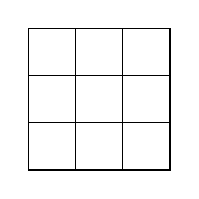
\begin{tikzpicture}[x=6mm,y=6mm, baseline={(current bounding box.center)}]
  \foreach \xy/\c in {(0,0)/white,(1,0)/white,(2,0)/white,
            (0,1)/white,(1,1)/white,(2,1)/white,
            (0,2)/white,(1,2)/white,(2,2)/white}
    \draw[fill=\c, shift={\xy}] (0,0) rectangle (1,1);
\end{tikzpicture}
  

Quatre instructions A, B, C et E permettent de changer l'aspect de certaines cases, lorsqu'on applique ces instructions. Ainsi:

\begin{tabularx}{\linewidth}{| >{\centering \arraybackslash}m{2cm} | m{8cm} | >{\centering \arraybackslash}X |} \hline
  Instruction & Descriptif & Effet de l'instruction   \\ \hline
  A &   La case centrale du motif est noircie.  & 
  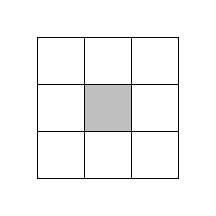
\begin{tikzpicture}[x=6mm,y=6mm, baseline={(current bounding box.center)}]
    \clip (-0.2,-0.2) rectangle (3.2,3.2);
    \foreach \xy/\c in {(0,0)/white,(1,0)/white,(2,0)/white,
      (0,1)/white,(1,1)/gray!50,(2,1)/white,
      (0,2)/white,(1,2)/white,(2,2)/white}
    \draw[fill=\c, shift={\xy}] (0,0) rectangle (1,1);
  \end{tikzpicture}  \\ \hline
  B &   Dans le motif, la case en bas à gauche et la case en haut à droite sont noircies. & 
      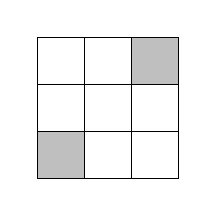
\begin{tikzpicture}[x=6mm,y=6mm, baseline={(current bounding box.center)}]
    \clip (-0.2,-0.2) rectangle (3.2,3.2);
    \foreach \xy/\c in {(0,0)/gray!50,(1,0)/white,(2,0)/white,
      (0,1)/white,(1,1)/white,(2,1)/white,
      (0,2)/white,(1,2)/white,(2,2)/gray!50}
    \draw[fill=\c, shift={\xy}] (0,0) rectangle (1,1);
  \end{tikzpicture}  \\ \hline
  
  C &   Dans le motif, la case médiane à gauche et la case médiane à droite sont noircies. & 
      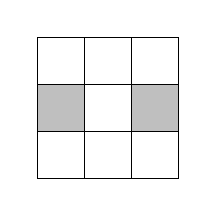
\begin{tikzpicture}[x=6mm,y=6mm, baseline={(current bounding box.center)}]
    \clip (-0.2,-0.2) rectangle (3.2,3.2);
    \foreach \xy/\c in {(0,0)/white,(1,0)/white,(2,0)/white,
      (0,1)/gray!50,(1,1)/white,(2,1)/gray!50,
      (0,2)/white,(1,2)/white,(2,2)/white}
    \draw[fill=\c, shift={\xy}] (0,0) rectangle (1,1);
  \end{tikzpicture}  \\ \hline
  
  
  E &  Les couleurs du motif sont inversées: les cases blanches deviennent noires et les les cases noires deviennent blanches.&
      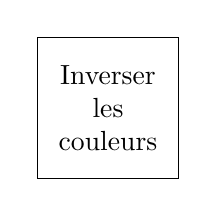
\begin{tikzpicture}[x=6mm,y=6mm, baseline={(current bounding box.center)}]
    \clip (-0.2,-0.2) rectangle (3.2,3.2);
    \draw[] (0,0) rectangle (3,3) ;
    \node (t) at (1.5,1.5) [text width=1.5cm, align=center] {Inverser\\ les\\ couleurs};
  \end{tikzpicture}  \\ \hline

\end{tabularx}


\emph{Remarque} : si une case du motif est déjà noire et une instruction demande de la noircir, alors cette case ne change pas de couleur et reste noire à la suite de cette instruction.


\emph{Exemples} : à partir d’un motif dont toutes les cases sont blanches:

\begin{tabularx}{\linewidth}{X c @{\hspace{5mm}}|@{\hspace{5mm}} X c} 
  la suite d'instructions A C permet d'obtenir ce motif &
  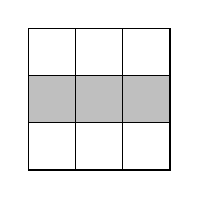
\begin{tikzpicture}[x=6mm,y=6mm, baseline={(current bounding box.center)}]
  \foreach \xy/\c in {(0,0)/white,(1,0)/white,(2,0)/white,
            (0,1)/gray!50,(1,1)/gray!50,(2,1)/gray!50,
            (0,2)/white,(1,2)/white,(2,2)/white}
    \draw[fill=\c, shift={\xy}] (0,0) rectangle (1,1);

  \end{tikzpicture}&
  la suite d'instructions A C E permet d'obtenir ce motif &
  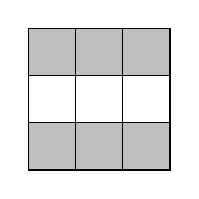
\begin{tikzpicture}[x=6mm,y=6mm, baseline={(current bounding box.center)}]
    \foreach \xy/\c in {(0,0)/gray!50,(1,0)/gray!50,(2,0)/gray!50,
            (0,1)/white,(1,1)/white,(2,1)/white,
            (0,2)/gray!50,(1,2)/gray!50,(2,2)/gray!50}
      \draw[fill=\c, shift={\xy}] (0,0) rectangle (1,1);
  \end{tikzpicture}\\		
\end{tabularx}


Pour chacune des questions suivantes, on dispose au départ d’un motif dont toutes les cases sont blanches.

\begin{enumerate}
  \item Représenter le motif obtenu avec la suite d'instructions A B.
  
  \item \begin{minipage}[t]{11 cm}
Parmi les quatre propositions suivantes, deux propositions permettent d'obtenir le motif ci-contre. Lesquelles ?
    
    \smallskip 
    
\begin{tabularx}{\linewidth}{*{2}{>{\bfseries Proposition \no }l <{ :} @{~} X}}
1 & A B C   & 3 & B C E C\\ [6pt]
2 & C E     & 4 & C A E A\\
\end{tabularx}
  \end{minipage}
  \hfill
  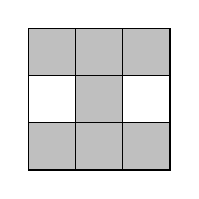
\begin{tikzpicture}[x=6mm,y=6mm, baseline={(0,1.6)}]
    \foreach \xy/\c in {(0,0)/gray!50,(1,0)/gray!50,(2,0)/gray!50,
              (0,1)/white,(1,1)/gray!50,(2,1)/white,
              (0,2)/gray!50,(1,2)/gray!50,(2,2)/gray!50}
      \draw[fill=\c, shift={\xy}] (0,0) rectangle (1,1);
  \end{tikzpicture}
  
  \item \begin{minipage}[t]{11 cm}
Donner une suite d'instructions qui permet d'obtenir le motif ci-contre.	
  \end{minipage}
  \hfill
%		\begin{tikzpicture}[x=6mm,y=6mm, baseline={(0,0.8)}]
%			\foreach \xy/\c in {(0,0)/gray!50,(1,0)/gray!50,(2,0)/white,
%								(0,1)/gray!50,(1,1)/white,(2,1)/gray!50,
%								(0,2)/white,(1,2)/gray!50,(2,2)/gray!50}
%			\draw[fill=\c, shift={\xy}] (0,0) rectangle (1,1);
%		\end{tikzpicture}
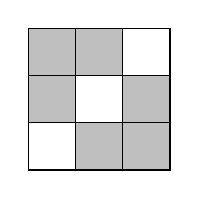
\begin{tikzpicture}[x=6mm,y=6mm, baseline={(0,0.8)}]
    \foreach \xy/\c in {(0,0)/white,(1,0)/gray!50,(2,0)/gray!50,
              (0,1)/gray!50,(1,1)/white,(2,1)/gray!50,
              (0,2)/gray!50,(1,2)/gray!50,(2,2)/white}
    \draw[fill=\c, shift={\xy}] (0,0) rectangle (1,1);
  \end{tikzpicture}
\end{enumerate}

\textbf{\textsc{Exercice 4 \hfill 8 points}}
\medskip

\begin{tabularx}{\linewidth}{|X|}\hline
Pour être en bonne santé, il est recommandé d'avoir régulièrement une pratique physique. Une recommandation serait de faire au moins une heure de pratique physique par jour en moyenne. Sur 1,6 million d'adolescents de 11 à 17 ans interrogés, 81\,\% d'entre eux ne respectent pas cette recommandation.\\ \hline
\end{tabularx}
\begin{flushright}\small {\emph{D'après un communiqué de presse sur la santé}}\end{flushright}
 
\begin{enumerate}
\item Sur les $1,6$ million d'adolescents de 11 à 17 ans interrogés, combien ne respectent pas cette recommandation ?
\end{enumerate}


Après la lecture de ce communiqué, un adolescent se donne un objectif.

\begin{center} \textbf{Objectif: \og  \emph{Faire au moins une heure de pratique physique par jour en moyenne.} \fg}\end{center}

Pendant 14 jours consécutifs, il note dans le calendrier suivant, la durée quotidienne qu'il consacre à sa pratique physique:

\begin{center} 
  \begin{tabularx}{\linewidth}{|*{7}{>{\centering \arraybackslash}X|}}\hline
  \textbf{Jour 1} 	&\textbf{Jour 2}&\textbf{Jour 3}		& \textbf{Jour 4}	&\textbf{Jour 5}	&\textbf{Jour} 6		&\textbf{Jour} 7\\ \hline
  50 min	&15 min&1 h			&1 h 40 min	&30 min	&1 h 30 min	&40 min\\ \hline
  \textbf{Jour 8}	&\textbf{Jour 9}&\textbf{Jour 10}		&\textbf{Jour 11}	&\textbf{Jour 12}&\textbf{Jour 13}	&\textbf{Jour 14}\\ \hline
  15 min	&1 h	&1 h 30 min	&30 min		&1 h 	&1 h 		&0 min\\ \hline
  \end{tabularx}
\end{center}

\begin{enumerate}[resume]
\item 
  \begin{enumerate}
    \item Quelle est l'étendue des 14 durées quotidiennes notées dans le calendrier ?
    \item Donner une médiane de ces 14 durées quotidiennes.
  \end{enumerate}
\item
  \begin{enumerate}
    \item En calculant la moyenne, montrer que, sur les 14 premiers jours, cet adolescent n'a pas atteint son objectif.
    \item  Pendant les 7 jours suivants, cet adolescent décide alors de consacrer plus de temps au sport pour atteindre son objectif sur l'ensemble des $21$ jours.

Sur ces 7 derniers jours, quelle est la durée totale de pratique physique qu'il doit au minimum prévoir pour atteindre son objectif?
  \end{enumerate}
\end{enumerate}

\textbf{\textsc{Exercice 5 \hfill 8 points}}


On souhaite rénover une salle de bain qui a la forme d’un parallélépipède rectangle. Il faut coller du papier peint sur les quatre murs. On n’en colle pas sur la porte, ni sur la fenêtre.
	
Voici un schéma de la salle de bain, les dimensions sont exprimées en mètre :
	
\begin{center}
	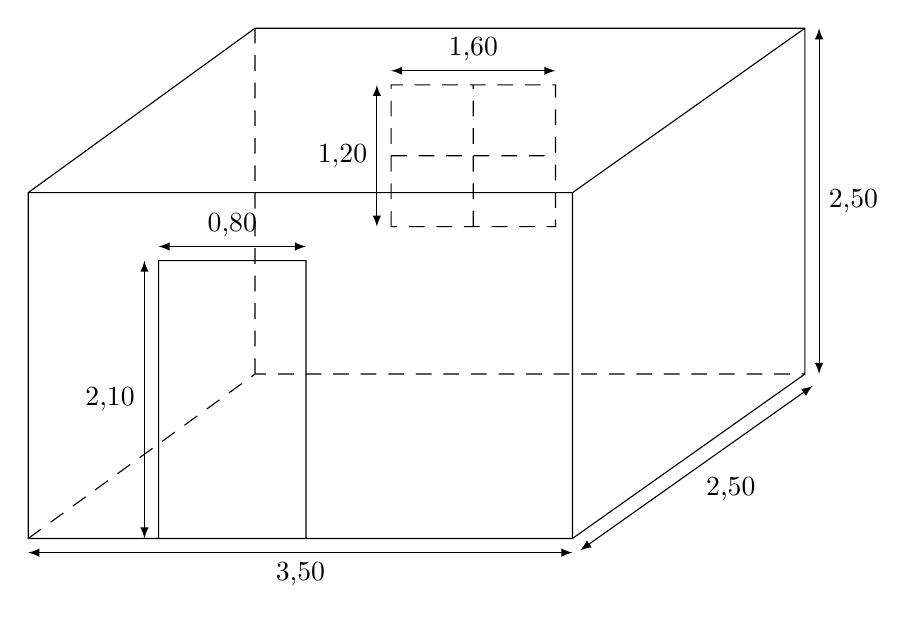
\begin{tikzpicture}[x=0.9cm,y=0.9cm,> = latex,scale=0.8]
		\draw  (0,0) rectangle (9.6,6.1)
			   (2.3,0) rectangle (4.9,4.9)	
			   (0,6.1)--(4,9)--(13.7,9)--(13.7,2.9)--(9.6,0)
			   (9.6,6.1)--(13.7,9);
		\draw[dash pattern=on 2mm off 1.5mm] 
				(0,0)--(4,2.9)--(13.7,2.9)
				(4,2.9)--(4,9)
				(6.4,5.5) rectangle (9.3,8)
				(7.85,5.5)--(7.85,8)
				(6.4,6.75)--(9.3,6.75);
		\draw[<->, shift={(0,-0.25)}] (0,0)--(9.6,0)
		node[below,pos=0.5]{3,50};
		\draw[<->, shift={(-57:0.25)}] (9.6,0)--(13.7,2.9)
		node[below right,pos=0.5]{2,50};
		\draw[<->, shift={(0.25,0)}] (13.7,2.9)--(13.7,9)
		node[right,pos=0.5]{2,50};
		\draw[<->, shift={(-0.25,0)}] (2.3,0)--(2.3,4.9)
		node[left,pos=0.5]{2,10};
		\draw[<->, shift={(0,0.25)}] (2.3,4.9)--(4.9,4.9)
		node[above,pos=0.5]{0,80};
		\draw[<->, shift={(-0.25,0)}] (6.4,5.5)--(6.4,8)
		node[left,pos=0.5]{1,20};
		\draw[<->, shift={(0,0.25)}] (6.4,8)--(9.3,8)
		node[above,pos=0.5]{1,60};
	\end{tikzpicture}
\end{center}
	
On dispose des informations suivantes :
	
\fbox{\rule[-2.1cm]{0mm}{4.4cm}\begin{minipage}{0.53\linewidth}
		Prix du papier peint :
			
		\begin{itemize}[label=\textbullet,leftmargin=*]
			\item le papier peint est vendu au rouleau entier ;
			
			\item un rouleau coûte 16,95 \euro{};
			\item un rouleau permet de recouvrir 5,3 m$^2$.
		\end{itemize}
		\emph{Conseil du vendeur :} 
			
		prévoir 1 rouleau de papier peint en plus afin de compenser les pertes liées aux découpes.
\end{minipage}}
\hfill
\fbox{\rule[-2.1cm]{0mm}{4.4cm}\begin{minipage}{0.42\linewidth}
	Prix de la colle :
	\begin{itemize}[label=\textbullet,leftmargin=*]
		\item la colle est vendue au pot entier ;
		\item un pot a une masse de 0,2 kg;
		\item un pot coûte 5,70 \euro{}.
	\end{itemize}
			\emph{Conseil du vendeur :}
		
	compter 1 pot de colle pour 4 rouleaux de papier peint.		
\end{minipage}}

\begin{enumerate}
	\item Montrer que la surface à recouvrir de papier peint est de 26,4 m$^2$.
	
	\item Calculer le prix, en euro, d’un mètre carré de papier peint.
	Arrondir au centime d'euro.
	
	\item Si on suit les conseils du vendeur, combien coûtera la rénovation de la salle de bain ?
		
	\item Le jour de l'achat, une remise de 8 \% est accordée.
		
	Quel est le prix à payer après remise ? Arrondir au centime d'euro.
\end{enumerate}

\end{document}